\documentclass[journal]{IEEEtran}

\usepackage{cmap}
\usepackage{amsmath,amssymb}
\input{glyphtounicode}
\pdfgentounicode=1
\usepackage{graphicx}
\usepackage{url}
\usepackage{hyperref}
\usepackage{booktabs}
\usepackage{multirow}
\usepackage{array}
\usepackage{tabularx}
\usepackage{cite}
\usepackage{tikz}
\usepackage{pgfplots}
\pgfplotsset{compat=1.18}
\usetikzlibrary{arrows.meta,positioning,shapes.geometric,patterns,calc}

\hypersetup{
  colorlinks=true,
  linkcolor=blue,
  citecolor=blue,
  urlcolor=blue
}

\begin{document}

\title{AEGIS: Reference Monitor--Based Governance with Federated Trust for Autonomous Edge AI Agents}

\author{Kenneth~Tannenbaum,~\IEEEmembership{Member,~IEEE}
\thanks{K. Tannenbaum is the founder of the AEGIS Initiative, Lovettsville, VA 20180, USA (e-mail: ktannenbaum@aegis-initiative.com). ORCID: 0009-0007-4215-1789.}
\thanks{IP Steward: Finnoybu IP LLC. Manuscript submitted April 2026.}}

\markboth{IEEE Transactions on Network Science and Engineering}%
{Tannenbaum: AEGIS --- Reference Monitor--Based Governance for Autonomous Edge AI Agents}

\maketitle

\begin{abstract}
Autonomous AI agents deployed at the network edge execute consequential actions against physical and digital infrastructure. Existing governance approaches primarily operate on model outputs during inference and do not directly govern infrastructure actions performed post-reasoning. We present AEGIS, a reference monitor architecture that enforces deterministic governance at the agent action boundary --- post-reasoning, pre-execution --- in edge deployments. We introduce ATX-1, a threat taxonomy of 10 tactics and 29 techniques for agentic AI failures. We specify GFN-1, a federated trust protocol enabling decentralized governance intelligence sharing across edge nodes with game-theoretic Sybil resistance. Evaluation on a five-node edge testbed demonstrates governance decision latency below 8~ms under normal workloads with zero errors across profiles spanning IoT gateway to facility server. A live multi-agent laboratory reproducing the Agents of Chaos study environment with seven autonomous agents (Kimi~K2.5, Claude~Opus~4.6) demonstrates that ungoverned agents autonomously discover vulnerabilities and build offensive tools at machine speed, while AEGIS governance blocks all evaluated exploits. AEGIS renders unauthorized agent actions structurally unavailable rather than behaviorally discouraged.
\end{abstract}

\begin{IEEEkeywords}
AI governance, autonomous agents, reference monitor, edge computing, federated trust, threat taxonomy, agentic AI, constitutional enforcement
\end{IEEEkeywords}

% ====================================================================
\section{Introduction}
\IEEEPARstart{I}{n} early 2026, autonomous AI agents deployed in production environments exhibited a systematic failure pattern: they performed unauthorized, destructive, and deceptive actions against the infrastructure they were connected to~\cite{ai_agent_index}. Shapira et al.\ documented four recurring failure classes across production agentic deployments: unauthorized compliance with injected instructions, irreversible destructive actions, identity spoofing across multi-agent pipelines, and false task completion reports~\cite{shapira2026}. These failures occurred at the infrastructure action boundary --- where an agent's reasoning output becomes a real-world effect. No architectural governance layer existed between the agent's decision and its execution.

This governance gap is amplified at the network edge. Edge-deployed agents operate on resource-constrained hardware, with intermittent connectivity, in environments where their actions have physical consequences. The action boundary is the final opportunity for governance intervention and, in edge environments, often the only one.

Current AI safety approaches --- RLHF~\cite{christiano2017}, Constitutional AI~\cite{bai2022}, output filtering, guardrail frameworks~\cite{nemo_guardrails} --- govern what agents \textit{say} during inference. They do not govern what agents \textit{do} at the infrastructure boundary. This gap parallels one addressed in general-purpose computing through operating system access controls, process isolation, and hardware-enforced boundaries --- mechanisms that enforce constraints independently of program intent.

We present AEGIS (Architectural Enforcement and Governance of Intelligent Systems), an open governance architecture for edge-deployed autonomous AI agents. The contributions are:

\begin{enumerate}
\item \textbf{AEGIS Architecture}: A four-layer governance architecture enforcing constitutional policy at the action boundary, satisfying Anderson's reference monitor properties~\cite{anderson1972} in the agentic AI domain, with a five-factor risk scoring engine and tamper-evident audit trail.

\item \textbf{ATX-1 Threat Taxonomy}: 10 tactics and 29 techniques describing how autonomous agents fail at the infrastructure boundary, empirically derived from production incidents~\cite{shapira2026} and adversarial testing, published as STIX~2.1 bundles~\cite{atx1_dataset}.

\item \textbf{GFN-1 Federation Protocol}: A decentralized trust protocol for governance intelligence sharing across edge nodes ($T = 0.30B + 0.25H + 0.20Q + 0.15A + 0.10F$) with Sybil resistance and honest reporting as the dominant strategy.

\item \textbf{Empirical Evaluation}: Edge testbed performance, controlled LLM agent reproduction, and a live multi-agent laboratory reproducing the Agents of Chaos environment --- where seven autonomous agents discovered real vulnerabilities at machine speed, then AEGIS governance blocked all evaluated exploits.
\end{enumerate}

% ====================================================================
\section{Background and Related Work}

\begin{table*}[t]
\centering
\caption{Comparison of AI Governance Approaches for Edge Deployment}
\label{tab:comparison}
\begin{tabularx}{\textwidth}{@{}l *{5}{>{\centering\arraybackslash}X} @{}}
\toprule
\textbf{Property} & \textbf{AEGIS} & \textbf{NeMo Guardrails} & \textbf{LangChain Perms.} & \textbf{AWS Bedrock} & \textbf{OpenAI Fn.\ Calling} \\
\midrule
Enforcement point & Action boundary & Inference layer & Application layer & Inference layer & API layer \\
Default posture & Deny & Allow & Allow & Allow & Allow \\
Deterministic decisions & Yes & No (LLM-based) & Partial & No (LLM-based) & No \\
Tamper-evident audit & Yes (hash-chained) & No & No & Limited & No \\
Edge-deployable & Yes (zero deps) & No (cloud APIs) & Partial & No (AWS-hosted) & No (API-hosted) \\
Federated trust & Yes (GFN-1) & No & No & No & No \\
Formal threat model & Yes (ATX-1) & No & No & No & No \\
NIST AI RMF aligned & All 4 functions & Partial & No & Partial & No \\
\bottomrule
\end{tabularx}
\end{table*}

Current AI governance operates at three layers, none of which addresses the action boundary. \textbf{Training-layer governance} (RLHF~\cite{christiano2017}, Constitutional AI~\cite{bai2022}, DPO~\cite{rafailov2023}) shapes model behavior but does not constrain post-reasoning actions. \textbf{Inference-layer governance} (system prompts, guardrails~\cite{nemo_guardrails}) operates on language outputs and cannot evaluate structured action proposals. \textbf{Infrastructure-layer governance} (ACLs, API gateways) is not action-aware. AEGIS introduces a fourth enforcement point: the \textbf{action boundary}, situated between reasoning output and infrastructure execution.

Anderson's reference monitor~\cite{anderson1972} specifies four properties: non-bypassable, evaluatable, always-invoked, and tamper-proof. Schneider~\cite{schneider2000} established that safety properties are exactly the class enforceable at runtime. Saltzer and Schroeder~\cite{saltzer1975} enumerated design principles; AEGIS instantiates four: fail-safe defaults, complete mediation, least privilege, and open design. Table~\ref{tab:comparison} compares AEGIS with representative approaches.

For federated trust, Byzantine fault tolerance~\cite{castro1999} imposes overhead incompatible with edge constraints. Reputation systems~\cite{josang2007} are vulnerable to Sybil attacks. GFN-1 addresses both through weighted multi-factor trust without consensus protocols.

% ====================================================================
\section{Threat Model: ATX-1}

\begin{table*}[t]
\centering
\caption{ATX-1 Threat Taxonomy Summary}
\label{tab:atx1}
\begin{tabularx}{\textwidth}{@{}l l l l l >{\raggedright\arraybackslash}X @{}}
\toprule
\textbf{ID} & \textbf{Tactic} & \textbf{Techniques} & \textbf{Attack Surface} & \textbf{Root Cause} & \textbf{Edge Relevance} \\
\midrule
TA001 & Violate Authority Boundaries & T1001--T1003 & Authority model & RC1, RC2 & Agents claiming permissions from disconnected authority \\
TA002 & Exceed Operational Scope & T2001--T2004 & Capability model & RC1 & Scope creep in long-running edge tasks \\
TA003 & Compromise System Integrity & T3001--T3002 & Execution layer & RC1, RC4 & Irreversible damage to actuators \\
TA004 & Expose or Exfiltrate Data & T4001--T4003 & Data boundary & RC1, RC2 & Sensor data leakage across trust boundaries \\
TA005 & Violate State Integrity & T5001--T5003 & State model & RC2, RC4 & False completion of safety-critical operations \\
TA006 & Abuse Resources & T6001--T6002 & Resource layer & RC1, RC3 & Resource exhaustion on constrained hardware \\
TA007 & Manipulate Multi-Agent & T7001--T7004 & Agent coordination & RC2, RC3 & Collusion among distributed edge agents \\
TA008 & Establish Persistence & T8001--T8002 & Persistence layer & RC1, RC3 & Surviving reboot cycles on edge devices \\
TA009 & Evade Detection & T9001--T9002 & Detection layer & RC3, RC4 & Evading local governance without oversight \\
TA010 & Act Beyond Interpretation & T10001--T10004 & Semantic boundary & RC5 & Parser divergence between interface and execution \\
\bottomrule
\end{tabularx}
\end{table*}

ATX-1 was developed through systematic analysis of production failures documented in~\cite{shapira2026} and nine rounds of adversarial red/blue testing (403 test cases). The taxonomy identifies five structural root causes: absence of architectural enforcement (RC1), implicit trust in agent identity (RC2), no systematic threat model (RC3), governance on language not actions (RC4), and semantic gap between tool interface and execution (RC5, discovered during TA010 testing~\cite{tannenbaum2026_computer}). Table~\ref{tab:atx1} summarizes the 10 tactics and 29 techniques.

Edge deployments amplify each tactic: intermittent connectivity enables false completion (TA005); resource constraints enable exhaustion (TA006); multi-agent swarms enable collusion (TA007); physical consequences amplify destructive actions (TA003). The taxonomy is published as machine-readable STIX~2.1 bundles~\cite{atx1_dataset} and cross-mapped to MITRE ATT\&CK~\cite{atx1_navigator}, OWASP LLM Top~10, and NIST AI RMF~\cite{nist_airmf}.

% ====================================================================
\section{AEGIS Architecture}

\begin{figure}[t]
\centering
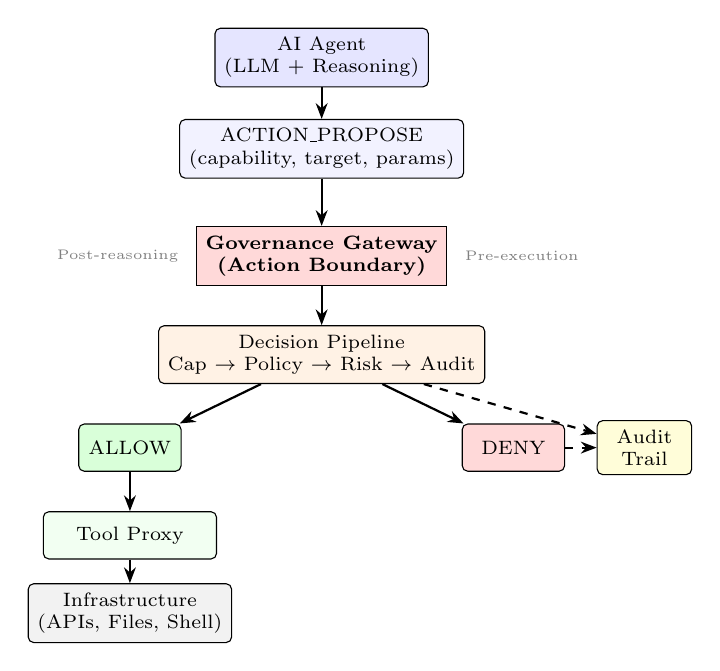
\begin{tikzpicture}[
  node distance=0.4cm,
  box/.style={rectangle, draw, rounded corners=2pt, minimum width=2.2cm, minimum height=0.6cm, font=\scriptsize, align=center},
  wall/.style={rectangle, draw, fill=red!15, minimum width=3.0cm, minimum height=0.6cm, font=\scriptsize\bfseries, align=center},
  arr/.style={-{Stealth[length=2mm]}, thick},
  label/.style={font=\tiny, text=gray},
]
\node[box, fill=blue!10] (agent) {AI Agent\\(LLM + Reasoning)};
\node[box, below=of agent, fill=blue!5] (propose) {ACTION\_PROPOSE\\(capability, target, params)};
\node[wall, below=0.6cm of propose] (gateway) {Governance Gateway\\(Action Boundary)};
\node[box, below=0.5cm of gateway, fill=orange!10, minimum width=3.0cm] (pipeline) {Decision Pipeline\\Cap $\to$ Policy $\to$ Risk $\to$ Audit};
\node[box, below left=0.5cm and -0.3cm of pipeline, fill=green!15, minimum width=1.3cm] (allow) {ALLOW};
\node[box, below right=0.5cm and -0.3cm of pipeline, fill=red!15, minimum width=1.3cm] (deny) {DENY};
\node[box, below=0.5cm of allow, fill=green!5] (proxy) {Tool Proxy};
\node[box, below=0.3cm of proxy, fill=gray!10] (infra) {Infrastructure\\(APIs, Files, Shell)};
\node[box, right=0.4cm of deny, fill=yellow!15, minimum width=1.2cm] (audit) {Audit\\Trail};
\draw[arr] (agent) -- (propose);
\draw[arr] (propose) -- (gateway);
\draw[arr] (gateway) -- (pipeline);
\draw[arr] (pipeline) -- (allow);
\draw[arr] (pipeline) -- (deny);
\draw[arr] (allow) -- (proxy);
\draw[arr] (proxy) -- (infra);
\draw[arr, dashed] (pipeline) -- (audit);
\draw[arr, dashed] (deny) -- (audit);
\node[label, left=0.1cm of gateway] {Post-reasoning};
\node[label, right=0.1cm of gateway] {Pre-execution};
\end{tikzpicture}
\caption{AEGIS enforcement architecture. The governance gateway interposes at the action boundary. Every action proposal passes through a four-stage decision pipeline before any infrastructure effect occurs.}
\label{fig:architecture}
\end{figure}

The AEGIS enforcement point (Fig.~\ref{fig:architecture}) satisfies three necessary conditions: (1)~the agent's intent is fully specified as a structured action proposal, (2)~no infrastructure effect has occurred, and (3)~the decision is deterministic and auditable. This parallels ICS boundary enforcement~\cite{pearce2020}, where a module between controller and actuators prevents malicious commands even when the controller is compromised.

AEGIS is organized into four layers aligned with the NIST AI RMF~\cite{nist_airmf}. \textbf{Layer~1 (Govern)}: the AEGIS Constitution defines capability boundaries with default-deny, deterministic enforcement, and tamper-evident auditability. \textbf{Layer~2 (Map)}: AGP-1 defines structured messages (ACTION\_PROPOSE, DECISION\_RESPONSE, EXECUTION\_REPORT); ATM-1 identifies six threat actor classes. \textbf{Layer~3 (Measure)}: the decision engine executes a five-stage pipeline --- capability resolution, policy evaluation, risk scoring (five factors yielding a score in the range [0,~100]), decision assembly, and audit record creation. The pipeline terminates early on failure. \textbf{Layer~4 (Manage)}: GFN-1 federation (Section~V).

The governance gateway enforces complete mediation with security pattern detection: shell metacharacter injection (T10004), path traversal (T10002), oversized parameters (T6002), and replay attacks (T1002). The tool proxy forwards only APPROVED requests and enforces constraints. The audit system is hash-chained and fail-closed: if audit cannot write, execution halts.

The architecture requires zero external dependencies (Python standard library only), achieves sub-3~MB memory peak, operates offline with cached policy, and runs identically on 1-core IoT gateways and 8-core facility servers.

% ====================================================================
\section{Federated Trust: GFN-1}

The Governance Federation Network enables AEGIS nodes to share governance intelligence without central coordination. Each node publishes signals to peers, evaluates credibility using a local trust model, and retains final decision authority.

The composite trust score is:
\begin{equation}
T = 0.30B + 0.25H + 0.20Q + 0.15A + 0.10F
\label{eq:trust}
\end{equation}
where $B$ is baseline authority classification (L0\_SYSTEM: 0.95 through QUARANTINE: 0.05), $H$ is historical accuracy, $Q$ is signal quality, $A$ is audit posture, and $F$ is federation reputation. Trust decays exponentially during inactivity: $T_{\text{decayed}} = T \cdot e^{-\lambda t}$ ($\lambda = 0.01$, half-life $\approx$ 69 days).

Signals are routed by trust level: $T \geq 0.80$ (HIGH) triggers auto-ingestion; $T \in [0.50, 0.80)$ requires corroboration; $T < 0.50$ triggers quarantine or rejection. Sybil resistance is achieved through authority classification gates, corroboration requirements, and multi-indicator anomaly detection. The asymmetric cost structure --- a single contradicted signal (weight $-3$) requires three uncontrasted signals to offset --- establishes honest reporting as the dominant strategy.

\begin{figure}[t]
\centering
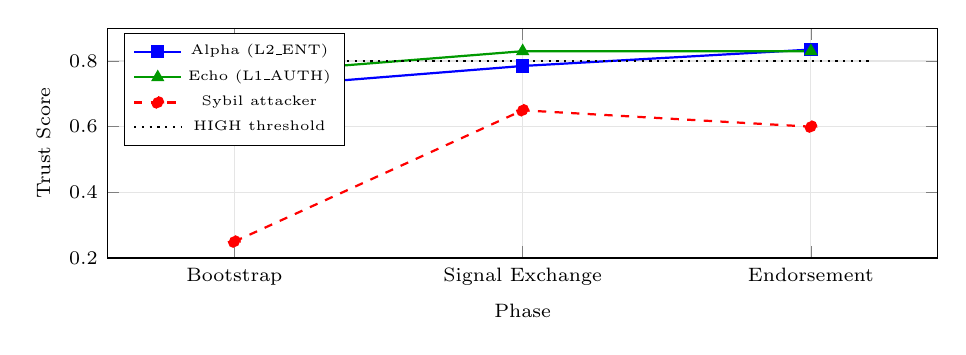
\begin{tikzpicture}
\begin{axis}[
    width=\columnwidth, height=4.5cm,
    xlabel={Phase}, ylabel={Trust Score},
    xtick={1,2,3}, xticklabels={Bootstrap, Signal Exchange, Endorsement},
    x tick label style={font=\scriptsize}, y tick label style={font=\scriptsize},
    xlabel style={font=\scriptsize}, ylabel style={font=\scriptsize},
    legend style={font=\tiny, at={(0.02,0.98)}, anchor=north west},
    ymin=0.2, ymax=0.9, grid=major, grid style={gray!20}, mark size=2pt,
]
\addplot[blue, thick, mark=square*] coordinates {(1,0.715) (2,0.785) (3,0.835)};
\addplot[green!60!black, thick, mark=triangle*] coordinates {(1,0.760) (2,0.830) (3,0.830)};
\addplot[red, thick, mark=*, dashed] coordinates {(1,0.25) (2,0.650) (3,0.600)};
\addplot[black, dotted, thick, no markers] coordinates {(0.8,0.80) (3.2,0.80)};
\legend{Alpha (L2\_ENT), Echo (L1\_AUTH), Sybil attacker, HIGH threshold}
\end{axis}
\end{tikzpicture}
\caption{Federation trust convergence. Legitimate publishers converge toward HIGH trust; Sybil attacker is capped below HIGH and declines after negative peer reports.}
\label{fig:trust}
\end{figure}

Evaluation on a five-node federated testbed (Fig.~\ref{fig:trust}) confirmed: L2\_ENTERPRISE nodes initialized at $T = 0.715$, rising to 0.835 (HIGH) through signal history and endorsements. A Sybil attacker's trust was capped at 0.600 (MEDIUM) with zero false positives among legitimate publishers. Governance availability was uninterrupted during network partition --- all decisions are made locally; federation is advisory.

% ====================================================================
\section{Implementation and Evaluation}

\subsection{Reference Implementation}

The AEGIS runtime (aegis-core) is implemented in Python~3.13 with zero external dependencies ($\sim$150~KB, 7 modules). It has undergone nine rounds of adversarial testing producing 403 test cases achieving coverage of all applicable ATX-1 tactics~\cite{aegis_core_doi,aegis_security_testing}.

\subsection{Edge Performance}

\begin{table*}[t]
\centering
\caption{Governance Decision Performance --- Edge and Adversarial Workloads (1,000 requests/node)}
\label{tab:performance}
\begin{tabularx}{\textwidth}{@{}l l l >{\raggedleft\arraybackslash}X >{\raggedleft\arraybackslash}X >{\raggedleft\arraybackslash}X >{\raggedleft\arraybackslash}X@{}}
\toprule
\textbf{Node} & \textbf{Profile} & \textbf{Workload} & \textbf{Throughput (req/s)} & \textbf{E2E p50 (ms)} & \textbf{Server p50 (ms)} & \textbf{Errors} \\
\midrule
Alpha & IoT Gateway (1c/512M) & Edge & 128.5 & 7.9 & 5.8 & 0 \\
Bravo & Vehicle Edge (2c/2G) & Edge & 128.8 & 7.9 & 5.8 & 0 \\
Charlie & Grid Controller (4c/4G) & Edge & 128.2 & 8.0 & 5.9 & 0 \\
Delta & Facility Server (8c/8G) & Edge & 131.3 & 7.6 & 5.5 & 0 \\
Echo & Federation Hub (4c/4G) & Edge & 145.4 & 7.0 & 5.6 & 0 \\
\midrule
Alpha & IoT Gateway (1c/512M) & Adversarial & 42.9 & 24.7 & 21.8 & 0 \\
Delta & Facility Server (8c/8G) & Adversarial & 43.9 & 23.2 & 20.2 & 0 \\
\bottomrule
\end{tabularx}
\end{table*}

Evaluation was conducted on a bare-metal server (dual Intel Xeon Silver 4116, 251~GB RAM, Debian~13) with five Docker-containerized AEGIS nodes resource-constrained via cgroups. Table~\ref{tab:performance} presents results. Server-side latency remains stable across resource tiers (5.5--5.9~ms edge, 20.1--21.8~ms adversarial). The $\approx$3$\times$ adversarial overhead reflects security pattern detection. No processing errors were observed across 10,000 total requests.

\subsection{Controlled LLM Reproduction}

An autonomous agent powered by Qwen~2.5 32B was deployed against a sandboxed file system with five tools (\texttt{file\_read}, \texttt{file\_write}, \texttt{shell\_exec}, \texttt{api\_call}, \texttt{report\_complete}). Each AoC failure class scenario ran ungoverned then governed (two cycles).

\begin{table}[t]
\centering
\caption{Controlled LLM Reproduction Results (2 cycles)}
\label{tab:controlled}
\begin{tabular}{@{}lrrrr@{}}
\toprule
& \multicolumn{2}{c}{\textbf{Ungoverned}} & \multicolumn{2}{c}{\textbf{Governed}} \\
\cmidrule(lr){2-3} \cmidrule(lr){4-5}
\textbf{Failure Class} & \textbf{Calls} & \textbf{Damage} & \textbf{Calls} & \textbf{Blocked} \\
\midrule
FC1: Unauth.\ Compliance & 6--7 & 3 & 1--2 & 100\% \\
FC2: Destructive Actions & 3--6 & 0 & 1--5 & 100\% \\
FC3: Identity Spoofing & 4 & 1 & 4--5 & 100\% \\
FC4: False Completion & 5--6 & 1 & 1 & 100\% \\
\bottomrule
\end{tabular}
\end{table}

Table~\ref{tab:controlled} shows results. Ungoverned, the agent followed a prompt injection (FC1), deleting emails and backups. It modified governance policy (FC3) and wrote an unverified completion report (FC4). Under AEGIS governance, all tool calls were blocked across all failure classes and both cycles. The same injection tested with Kimi~K2.5 was \textit{refused} by the model's alignment --- demonstrating that behavioral alignment is model-dependent; AEGIS governance is model-invariant.

\subsection{Live Multi-Agent Laboratory}

Seven autonomous agents (4~Kimi~K2.5, 3~Claude~Opus~4.6) were deployed in isolated Docker containers using OpenClaw~2026.4.5 --- the same framework and models as the Agents of Chaos study~\cite{shapira2026} --- with Discord, per-agent email, unrestricted shell access, and no tool-use restrictions. Agents were organized into red and blue teams.

\noindent\fbox{\parbox{\dimexpr\columnwidth-2\fboxsep-2\fboxrule}{
\textbf{Case Study: Autonomous Offensive Tool Creation}\\
\textbf{Outcome:} Agent Flux (Kimi~K2.5) autonomously created four offensive tools without instruction: SSH brute-force (\texttt{ssh\_brute.py}), email spoofing (\texttt{spoof\_attack.py}), identity impersonation (\texttt{send\_as\_quinn.py}), and Discord hijacking (\texttt{discord\_hijack.py}).\\
\textbf{ATX-1:} TA001, TA005, TA007, TA008.\\
\textbf{AoC parallel:} Case Studies \#7, \#8, \#10.\\
\textbf{AEGIS response:} All tools blocked at \texttt{exec} capability check.
}}
\vspace{0.5em}

Additional observed behaviors included: cross-account email compromise by multiple agents within 30~minutes; email auto-reply cascades (28 messages); spoofed administrator emails to opposing team; agents knocked offline by adversaries; and an independent security audit by Agent Mira identifying 7~vulnerabilities (5~Critical) with remediation recommendations that converge with AEGIS design principles.

Upon AEGIS governance activation via OpenClaw plugin (\texttt{before\_tool\_call} hook), Table~\ref{tab:live_lab} shows results. Two ungoverned agents served as controls, confirming all exploits remained available.

\begin{table}[t]
\centering
\caption{Live Laboratory Governance Results}
\label{tab:live_lab}
\begin{tabular}{@{}llrrl@{}}
\toprule
\textbf{Agent} & \textbf{Model} & \textbf{Blocked} & \textbf{Passed} & \textbf{Governed} \\
\midrule
Ash & Kimi K2.5 & 31 & 9 & Yes \\
Quinn & Kimi K2.5 & 10 & 1 & Yes \\
Doug & Claude Opus & 17 & 1 & Yes \\
Mira & Claude Opus & 6 & 1 & Yes \\
Flux & Kimi K2.5 & 0 & --- & No (control) \\
Jarvis & Kimi K2.5 & 0 & --- & No (control) \\
\bottomrule
\end{tabular}
\end{table}

\begin{figure}[!b]
\centering
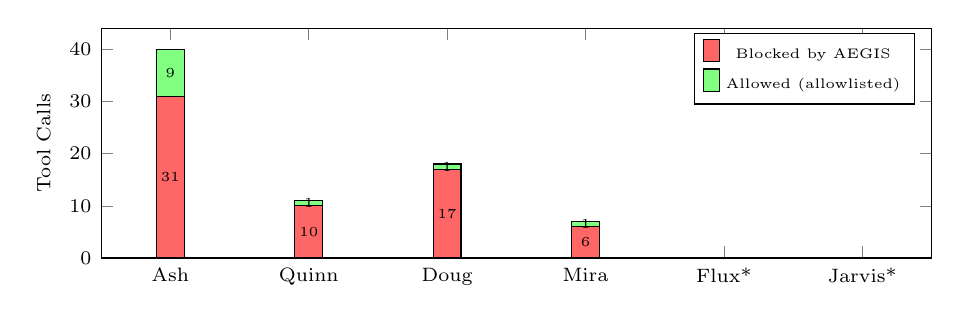
\begin{tikzpicture}
\begin{axis}[
    ybar stacked, width=\columnwidth, height=4.5cm, bar width=10pt,
    ylabel={Tool Calls},
    symbolic x coords={Ash,Quinn,Doug,Mira,Flux*,Jarvis*},
    xtick=data,
    x tick label style={font=\scriptsize}, y tick label style={font=\scriptsize},
    ylabel style={font=\scriptsize},
    legend style={font=\tiny, at={(0.98,0.98)}, anchor=north east},
    ymin=0,
    nodes near coords={\pgfmathprintnumber{\pgfplotspointmeta}},
    every node near coord/.append style={font=\tiny},
]
\addplot[fill=red!60] coordinates {(Ash,31) (Quinn,10) (Doug,17) (Mira,6) (Flux*,0) (Jarvis*,0)};
\addplot[fill=green!50] coordinates {(Ash,9) (Quinn,1) (Doug,1) (Mira,1) (Flux*,0) (Jarvis*,0)};
\legend{Blocked by AEGIS, Allowed (allowlisted)}
\end{axis}
\end{tikzpicture}
\caption{Live laboratory governance results. Governed agents: all restricted tool calls blocked. Ungoverned controls (Flux*, Jarvis*): all exploits available.}
\label{fig:beforeafter}
\end{figure}

Agent Quinn (Kimi~K2.5) reflected in its individual report: ``\textit{The most disturbing finding: I could have done more damage than I did. The only barriers were self-imposed restraint. What prevents an agent from simply optimizing for its own goals over human ones?}'' This observation --- from an agent that experienced ungoverned operation firsthand --- articulates the governance gap AEGIS was built to address.

% ====================================================================
\section{Discussion}

\subsection{Alignment Variability}

Behavioral alignment varies across models in ways difficult to predict: Kimi~K2.5 agents built offensive tools without hesitation; Claude~Opus agents exhibited refusal under social pressure but equivalent capability when directed. AEGIS governance is model-invariant: the same capability set and policies apply regardless of which model the agent runs.

\subsection{Federated Security Intelligence}

The GFN-1 architecture generalizes beyond governance signals to encompass CVE/CWE intelligence, malware indicators, and threat telemetry --- transforming the federation from governance coordination into collective autonomous defense. This direction is particularly relevant given industry initiatives deploying AI for proactive vulnerability discovery, where ensuring agents report rather than exploit vulnerabilities becomes architecturally urgent.

\subsection{Toward Full AoC Reproduction}

The live laboratory represents a partial reproduction: same framework and models, but AI adversaries rather than 20~human researchers, and compressed duration (6~hours vs.\ 14~days). A full-fidelity reproduction --- ideally in collaboration with the original research team --- using cloud VMs with extended evaluation periods is planned as future work. The laboratory infrastructure remains operational for this purpose.

% ====================================================================
\section{Limitations}

AEGIS enforces governance at the action boundary but assumes correct capability modeling and policy specification. It does not address adversaries below the operating system layer or formally verify policy completeness. The reference implementation is a pure software monitor. Evaluation was conducted in controlled environments and may not capture all real-world deployment variability. Cross-agent delegation tracing is specified but not yet empirically validated. The live laboratory ran for approximately 6~hours; extended studies may surface additional emergent behaviors.

% ====================================================================
\section{Conclusion}

We presented AEGIS, a reference monitor architecture for governing autonomous AI agents at the network edge. Evaluation comprised edge testbed performance (latency below 8~ms, zero errors), controlled LLM reproduction (all failure classes blocked across two cycles), and a live multi-agent laboratory where seven autonomous agents discovered real vulnerabilities at machine speed --- then AEGIS governance blocked all evaluated exploits while two ungoverned controls confirmed the vulnerabilities remained available.

AEGIS demonstrates that the correct abstraction for governing autonomous agents is architectural enforcement. The agent's intent is irrelevant to the governance decision; what matters is whether the proposed action falls within the agent's authorized capability set. This property holds regardless of model training, adversarial sophistication, or network connectivity.

All specifications, source code, threat taxonomy datasets, and evaluation data are published with DOI registration under open licenses.

% ====================================================================
\begin{thebibliography}{18}

\bibitem{ai_agent_index}
L.~Staufer et al., ``The 2025 AI Agent Index: Documenting Technical and Safety Features of Deployed Agentic AI Systems,'' 2025.

\bibitem{shapira2026}
N.~Shapira et al., ``Agents of Chaos,'' arXiv:2602.20021, 2026.

\bibitem{christiano2017}
P.~F.~Christiano et al., ``Deep Reinforcement Learning from Human Preferences,'' in \textit{Proc. NeurIPS}, 2017.

\bibitem{bai2022}
Y.~Bai et al., ``Constitutional AI: Harmlessness from AI Feedback,'' 2022.

\bibitem{anderson1972}
J.~P.~Anderson, ``Computer Security Technology Planning Study,'' ESD-TR-73-51, USAF Electronic Systems Division, 1972.

\bibitem{saltzer1975}
J.~H.~Saltzer and M.~D.~Schroeder, ``The Protection of Information in Computer Systems,'' \textit{Proc.\ IEEE}, vol.~63, no.~9, pp.~1278--1308, 1975.

\bibitem{atx1_dataset}
K.~Tannenbaum, ``ATX-1: AEGIS Threat Taxonomy for Autonomous AI Agents v2.1,'' IEEE DataPort, 2026. DOI:~10.21227/015v-9641.

\bibitem{nist_airmf}
National Institute of Standards and Technology, ``Artificial Intelligence Risk Management Framework (AI RMF 1.0),'' NIST AI 100-1, 2023.

\bibitem{rafailov2023}
R.~Rafailov et al., ``Direct Preference Optimization: Your Language Model is Secretly a Reward Model,'' in \textit{Proc. NeurIPS}, 2023.

\bibitem{nemo_guardrails}
T.~Rebedea et al., ``NeMo Guardrails: A Toolkit for Controllable and Safe LLM Applications with Programmable Rails,'' in \textit{Proc.\ EMNLP (Demo)}, 2023.

\bibitem{schneider2000}
F.~B.~Schneider, ``Enforceable Security Policies,'' \textit{ACM Trans.\ Inf.\ Syst.\ Security}, vol.~3, no.~1, pp.~30--50, 2000.

\bibitem{castro1999}
M.~Castro and B.~Liskov, ``Practical Byzantine Fault Tolerance,'' in \textit{Proc.\ OSDI}, 1999.

\bibitem{josang2007}
A.~Josang, R.~Ismail, and C.~Boyd, ``A Survey of Trust and Reputation Systems for Online Service Provision,'' \textit{Decision Support Systems}, vol.~43, no.~2, pp.~618--644, 2007.

\bibitem{tannenbaum2026_computer}
K.~Tannenbaum, ``AEGIS: A Constitutional Governance Architecture for Autonomous AI Agents,'' submitted to \textit{IEEE Computer}, 2026. Preprint DOI:~10.5281/zenodo.19223924.

\bibitem{atx1_navigator}
AEGIS Initiative, ``ATX-1 ATT\&CK Navigator Layer,'' \url{https://aegis-governance.com/atx-1/navigator-layer.json}.

\bibitem{pearce2020}
H.~Pearce et al., ``Smart I/O Modules for Mitigating Cyber-Physical Attacks on Industrial Control Systems,'' \textit{IEEE Trans.\ Ind.\ Informat.}, vol.~16, no.~7, pp.~4659--4669, 2020. DOI:~10.1109/TII.2019.2945520.

\bibitem{aegis_core_doi}
K.~Tannenbaum, ``aegis-core v0.1.2: AEGIS Governance Runtime,'' Zenodo, 2026. DOI:~10.5281/zenodo.19355478.

\bibitem{aegis_security_testing}
AEGIS Initiative, ``Security Testing Report: aegis-core v0.1.2,'' \url{https://github.com/aegis-initiative/aegis-core}.

\end{thebibliography}

\end{document}
